\documentclass[
    9pt,
    % draft,
    hyperref={bookmarks=false, colorlinks=false}, % urlcolor=blue,, ,
    xcolor={dvipsnames},
]{beamer}
%\includeonlyframes{current}

\usetheme[height=8mm]{Rochester} % Main Theme
\usecolortheme{default} % Color Theme

\usepackage{lmodern} % Optional to remove font size warnings
\DeclareMathOperator{\Tr}{Tr}

% === Numbering For amsthm theorem environments ===
\usepackage{xparse}
\usepackage{ifthen} % For checking optional parameters

\newcommand{\bs}[1]{\left[ #1 \right]} % brackets square
\newcommand{\br}[1]{\left( #1 \right)} % brackets round
\newcommand{\bc}[1]{\left\{ #1 \right\}} % brackets curly

% === Mathematical operators that are denoted with words ===

\newcommand{\tikzglobalposition}[4]{
    \begin{tikzpicture}[remember picture, overlay,scale=#1]
        \tikzset{shift={(current page.center)},xshift=#2\paperwidth,yshift=#3\paperheight}
        #4
    \end{tikzpicture}
}

\usepackage[warningthreshold=0.95]{resizegather} % For resizing gather environment to fit massive equations
\AtBeginNote{\scriptsize} % Make notes small
% \setbeameroption{show notes} % Shows notes
% \setbeameroption{show only notes} % Shows only notes
% \setbeameroption{show notes on second screen}
\usefonttheme[onlymath]{serif} % For serif font in math mode
\usepackage[backend=biber, style=verbose, doi=false, isbn=false, url=true]{biblatex} %
\usepackage{tabu}
\usepackage{silence}
\WarningFilter{biblatex}{Patching footnotes failed}
\renewcommand\mkbibacro[1]{{\footnotesize\MakeUppercase{#1}}} % http://tex.stackexchange.com/questions/203111/small-caps-font-warning-in-beamer-using-biblatex \tabulinesep=1.2mm
\setbeamertemplate{bibliography item}{\insertbiblabel}
\addbibresource{references.bib}
\AtBeginBibliography{\small}

\setbeamertemplate{navigation symbols}{
    \insertslidenavigationsymbol%
    \insertframenavigationsymbol%
    \insertsubsectionnavigationsymbol%
    \insertsectionnavigationsymbol%
    \insertdocnavigationsymbol%
    \insertbackfindforwardnavigationsymbol%
    \hspace{1em}%
    \usebeamerfont{footline} \insertframenumber/\inserttotalframenumber%
}

% https://tex.stackexchange.com/questions/44983/beamer-removing-headline-and-its-space-on-a-single-frame-for-plan-but-keepin?utm_medium=organic&utm_source=google_rich_qa&utm_campaign=google_rich_qa
\makeatletter
    \newenvironment{withoutheadline}{
        \setbeamertemplate{headline}[default]
        \def\beamer@entrycode{\vspace*{-\headheight}}
    }{}
\makeatother

\setbeamercolor{alerted text}{fg=yellow}

\usepackage{youngtab}
\usepackage{physics}
\usepackage{mathtools}

\newcommand{\incstr}[1]{\vcenter{\hbox{\includegraphics[scale=0.65]{figures/#1}}}} % including string diagrams

\title[]{The Quantum Marginals Problem}
\date[]{March 6, 2020}
\AtBeginSection[]{
  \begin{withoutheadline}
  \begin{frame}
  \vfill
  \centering
  \begin{beamercolorbox}[sep=8pt,center,shadow=false,rounded=false]{frametitle}
    {\large \insertsectionhead\par}
  \end{beamercolorbox}
  \vfill
  \end{frame}
  \end{withoutheadline}
}
\begin{document}

\nocite{*}

\begin{withoutheadline}
    \begin{frame}
        \titlepage
        \begin{center}
            {TC Fraser} \\
            \vspace{0.8em}
            {Quantum Foundations Group Meeting}
        \end{center}
    \end{frame}
\end{withoutheadline}

\begin{frame}
    \frametitle{Overview}
    \begin{enumerate}
        \item Big Picture \& Origins of the Problem
        \item Definitions and Terminology
        \item Various Applications and Known Results
        \item Quantum Causality \& The Future of Marginal Problems
    \end{enumerate}
\end{frame}

\section{Big Picture}
\begin{frame}
    \frametitle{Big Picture}
    % constraining local data which is compatible with a global model
    \begin{columns}
        \begin{column}{0.7\textwidth}
            \begin{itemize}
                \item When is local information compatible with a global model?
                \item Already many instances within Quantum Foundations
                \item Classical marginal problems (application to database integrity, knowledge integration, coalition games)\footnotemark{}
                \item Local operational data is contextual when in fails to admit of a global noncontextual ontological model\footnotemark{} 
                \item Wigner functions arise when trying to view the statistics of local quantum observables as marginals of a covariant global distribution 
            \end{itemize}
        \end{column}
        \begin{column}{0.3\textwidth}
            \begin{center}
                Example: \\
                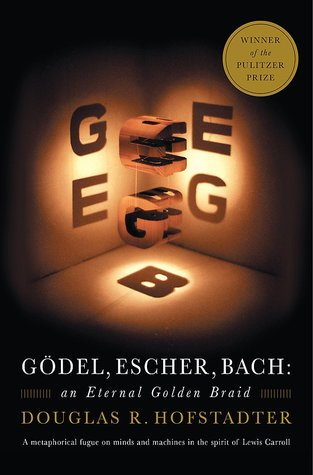
\includegraphics[width=\textwidth]{figures/geb_cover.jpg}
            \end{center}
        \end{column}
    \end{columns}
    \footcitetext{fritz2012entropic}
    \footcitetext{abramsky2011sheaf}
\end{frame}

\begin{frame}
    \frametitle{Origins of the Quantum Marginal Problem}
    \begin{columns}
        \begin{column}{0.6\textwidth}
            \begin{itemize}
                \item Originally appeared with application to quantum chemistry\footnotemark{}
                \item Consider a state of $N$-fermions $\ket{\psi} \in \bigwedge^N \mathcal H$
                \item and any $2$-local Hamiltonian
                    \[ H = \sum_{1 \leq i \leq N} h_i + \sum_{1 \leq i < j \leq N} h_{ij} \]
                \item Energetics of a state $\ket{\psi}\bra{\psi}$ only depend on reduced densities
                    \[ \Tr ( H \ket{\psi}\bra{\psi} ) = \sum_{1 \leq i < j \leq N} \Tr ( \tilde h_{ij} \rho_{ij} ) \]
            \end{itemize}
        \end{column}
        \begin{column}{0.4\textwidth}
            \begin{alertblock}{}
                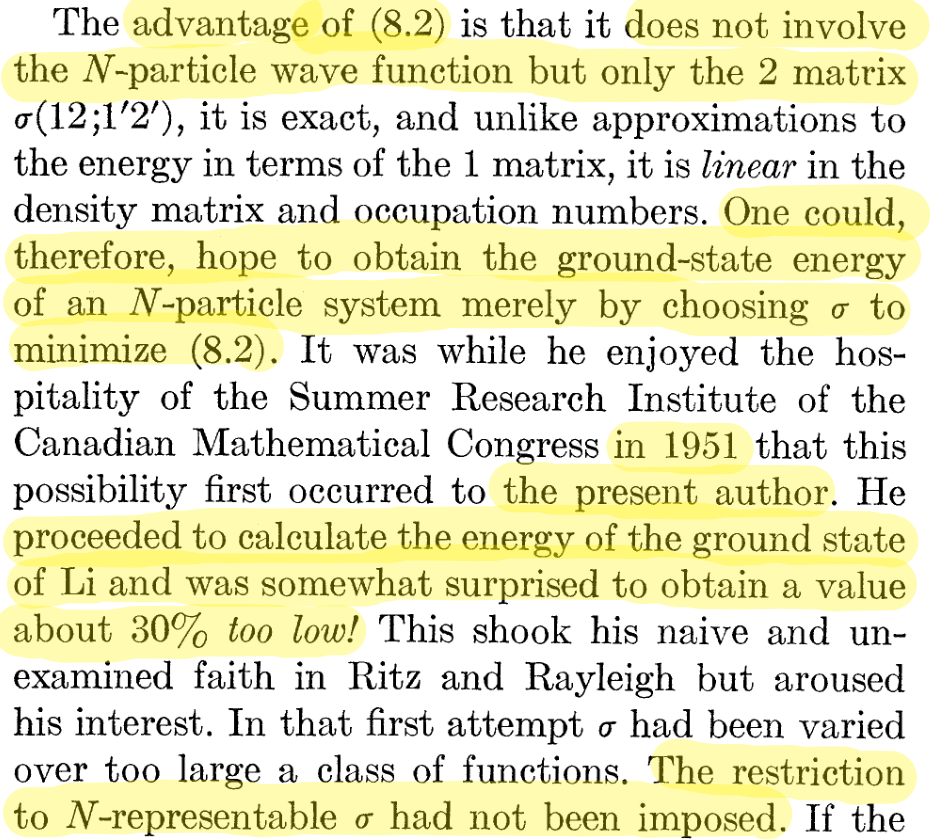
\includegraphics[width=\textwidth]{figures/coleman.png}
                \hspace*\fill{\small--- A. J. Coleman, 1963}
            \end{alertblock}
        \end{column}
    \end{columns}
    \begin{itemize}
        \item The \textit{$N$-representability problem} aims to characterize the space of $2$-body density operators which can be realized as the reduced states of an $N$-body fermionic pure state
    \end{itemize}
    \footcitetext{coleman1963structure}
\end{frame}

\begin{frame}
    \frametitle{The $N$-Representability Problem is Hard}
    \begin{alertblock}{}
        \textit{``We make no apology for the consideration of such a special case. The general $N$-representability problem for one and two body reduced density matrices is so difficult and yet so fundamental to many branches of science that each concrete result is useful in shedding light on the nature of the solution of the more general problem.''}
        \hspace*\fill{\small--- B. E. Borland, K. Dennis\footnotemark{}}
    \end{alertblock}
    \footcitetext{borland1972conditions}
    \begin{itemize}
        \item The $N$-representability problem is QMA-complete\footcite{liu2007quantum}.
    \end{itemize}
\end{frame}

\section{Terminology}
\begin{frame}
    \frametitle{The Quantum Marginals Problem: Terminology}
    \begin{columns}
        \begin{column}{0.6\textwidth}
            \begin{center}
                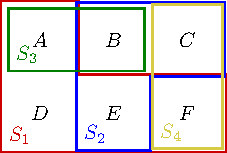
\includegraphics{figures/qmp_example.pdf}
            \end{center}
        \end{column}
        \begin{column}{0.4\textwidth}
            \begin{align*}
                \mathcal T &= \{ A, B, C, D, E, F \} \\
                S_1 &= \{ A, D, E, F \} \\
                S_2 &= \{ B, C, E \} \\
                S_3 &= \{ A, B \} \\
                S_4 &= \{ C, F \}
            \end{align*}
        \end{column}
    \end{columns}
    \begin{definition}
        A \textbf{quantum marginals problem (QMP)} can be identified by a family of subsystems $\{S_1,S_2, \ldots, S_m\} \in 2^{\mathcal T}$ of some total system $\mathcal T$. \\ 
        The objective is to characterize the space of families of density operators $\{\rho_{S_1}, \rho_{S_2}, \ldots, \rho_{S_m}\}$ with $\rho_{S_j} \in \mathcal B (\mathcal H_{S_j})$ for which
        \[ \text{there exists} \quad \rho_{\mathcal T} \in \mathcal B(\mathcal H_{\mathcal{T}}) \quad \text{such that} \quad \forall j : \Tr_{\mathcal T \setminus S_j}(\rho_{\mathcal T}) = \rho_{S_j} \] 
    \end{definition}
\end{frame}

\begin{frame}
    \frametitle{Variations of the Quantum Marginals Problem}
    \begin{itemize}
        \item \textit{pure} QMP : joint density operator $\rho_{\mathcal T} = \ket{\psi_{\mathcal T}}\bra{\psi_{\mathcal T}}$ is pure
        \item \textit{disjoint/univariate} QMP : the subsystems do not overlap $S_i \cap S_j = \delta_{ij} S_i$
        \item \textit{spectral} QMP : characterize the space of specta $\lambda_j  = \mathrm{spec}(\rho_{S_j})$
        \item \textit{fermionic} QMP : the joint density operator is $\rho_{\mathcal T} \in \mathcal B ( \bigwedge^{\abs{\mathcal T}} \mathcal H)$
        \item \textit{Gaussian} QMP : the marginal $\rho_{S_j}$ and joint density operators are Gaussian states
        \item \textit{channel} QMP : replace density operators with quantum channels
        \item and many more
    \end{itemize}
\end{frame}

\section{Results About the Disjoint Spectral QMP}
\begin{frame}
    \frametitle{Pure Marginal Problem for $N$ Qubits}
    \begin{theorem}[Higuchi-Sudbery-Szulc, 2003\footnotemark{}]
        For $N$ qubits $\otimes_{i=1}^{N} \mathcal H_i$ ($\mathrm{dim}(\mathcal H_i) = 2$), all constraints on the margins $\{ \rho_i \}_{i=1}^{n}$ of a pure state are given by 
        \[ \lambda_i \leq \sum_{j \neq i} \lambda_i \]
        where $\lambda_i$ is the minimal eigenvalue of $\rho_i$.
    \end{theorem}
    \footcitetext{higuchi2003one}
\end{frame}

\begin{frame}
    \frametitle{Mixed Spectral Marginal Problem for $2$ Qubits}
    \begin{theorem}[Bravyi, 2003\footnotemark{}]
        For $2$ qubits $\mathcal H_A \otimes \mathcal H_B$, the spectral marginal problem for $\{ A, B, AB \}$ is solved by 
        \begin{align*}
            \mathrm{min}(\lambda_A, \lambda_B) &\geq \lambda_3^{AB} + \lambda_4^{AB}, \\
            \lambda_A + \lambda_B &\geq \lambda_2^{AB} + \lambda_3^{AB} + 2\lambda_4^{AB}, \\
            |\lambda_A - \lambda_B| &\leq \mathrm{min}(\lambda_1^{AB} - \lambda_3^{AB}, \lambda_2^{AB} - \lambda_4^{AB}),
        \end{align*}
        where $\lambda_A, \lambda_B$ are minimal eigenvalues of $\rho_A, \rho_B$ and $\lambda_1^{AB} \geq \lambda_{2}^{AB} \geq \lambda_{3}^{AB} \geq \lambda_{4}^{AB}$ is the spectrum of $\rho_{AB}$.
    \end{theorem}
    \footcitetext{bravyi2003requirements}
\end{frame}

\begin{frame}
    \frametitle{Pure Spectral Marginal Problem for $3$ Qutrits}
    \begin{theorem}[Higuchi, 2003\footnotemark{}]
        For $3$ qutrits $\mathcal H_1 \otimes \mathcal H_2 \otimes \mathcal H_3$  ($\mathrm{dim}(\mathcal H_i) = 3$), a necessary and sufficient condition on the nine spectral values $0 \leq \lambda_1^{(a)} \leq \lambda_2^{(a)} \leq \lambda_3^{(a)}$ and $\lambda_1^{(a)} + \lambda_2^{(a)} + \lambda_3^{(a)} = 1$ for $a = 1,2,3$ to be the reduced spectra of a pure three-qutrit quantum state is given by the following:
        \begin{align*}
            \lambda_2^{(a)} + \lambda_1^{(a)} &\leq \lambda_2^{(b)} + \lambda_1^{(b)} + \lambda_2^{(c)} + \lambda_1^{(c)}, \\
            \lambda_3^{(a)} + \lambda_1^{(a)} &\leq \lambda_2^{(b)} + \lambda_1^{(b)} + \lambda_3^{(c)} + \lambda_1^{(c)}, \\
            \lambda_2^{(a)} + \lambda_3^{(a)} &\leq \lambda_2^{(b)} + \lambda_1^{(b)} + \lambda_2^{(c)} + \lambda_3^{(c)}, \\
            2\lambda_2^{(a)} + \lambda_1^{(a)} &\leq 2\lambda_2^{(b)} + \lambda_1^{(b)} + 2\lambda_2^{(c)} + \lambda_1^{(c)}, \\
            2\lambda_1^{(a)} + \lambda_2^{(a)} &\leq 2\lambda_2^{(b)} + \lambda_1^{(b)} + 2\lambda_1^{(c)} + \lambda_2^{(c)}, \\
            2\lambda_2^{(a)} + \lambda_3^{(a)} &\leq 2\lambda_2^{(b)} + \lambda_1^{(b)} + 2\lambda_2^{(c)} + \lambda_3^{(c)}, \\
            2\lambda_2^{(a)} + \lambda_3^{(a)} &\leq 2\lambda_1^{(b)} + \lambda_2^{(b)} + 2\lambda_3^{(c)} + \lambda_2^{(c)},
        \end{align*}
        where $(abc)$ are any permutations of $(123)$.
    \end{theorem}
    \footcitetext{higuchi2003qutrit}
\end{frame}

\begin{frame}
    \frametitle{Klyachko Shows Us the Light}
    \begin{itemize}
        \item In 2004\footcite{klyachko2004quantum} and 2006\footcite{klyachko2006quantum}, \citeauthor{klyachko2006quantum} effectively solves all disjoint spectral QMP
        \item Utilizes results from \textit{geometric invariant theory}, in particular the Hilbert-Mumford stability criterion to derive necessary and sufficient constraints on spectra\footcite{ressayre2010geometric}.
        \item Essential conclusion: the space of compatible disjoint spectra is always a finite polytope!
        \item Also applies to the spectra of the Riemann curvature tensor $\mathrm{R} : \wedge^2 \mathcal T \to \wedge^2 \mathcal T$ and Ricci tensor $\mathrm{Ric} : \mathcal T \to \mathcal T$ which are mutually compatible (inequalities are unpublished, but in his slides)
        \item Establishes connection with representation theory using \citeauthor{berenstein2000coadjoint}'s work\footcite{berenstein2000coadjoint}
    \end{itemize}
    \begin{alertblock}{}
        \textit{``For overlapping margins like $\rho_{AB}, \rho_{BC}, \rho_{AC}$, the problem is beyond the scope of the current approach.''}
        \hspace*\fill{\small--- A. Klyachko, 2009}
    \end{alertblock}
\end{frame}

\begin{frame}
    \frametitle{Notable PhD Theses}
    \begin{itemize}
        \item \citeauthor{schilling2015quantum}'s thesis\footcite{schilling2015quantum}: 
            \begin{itemize}
                \item Greatly elaborates and expands upon the mathematical formalism behind Klyachko's approach
                \item Ephasizes the importance of variational principles (Ky-Fan, Hersch-Zwahlen)
                \item Develops the physical inuition behind Klyachko's solution to the fermionic $N$-representability in terms of \textit{generalized Pauli constraints} and \textit{(quasi-)pinning}.
            \end{itemize}
        \item \citeauthor{klassen2017existence}'s thesis\footcite{klassen2017existence}:
            \begin{itemize}
                \item Investigates the extent to which various features of the global quantum state can be uniquely determined by its marginals.
            \end{itemize}
    \end{itemize}
\end{frame}

\section{Connections to the Representation Theory of $S_k$}
\begin{frame}
    \frametitle{Estimating the Spectra of a Density Operator}
    \begin{columns}
        \begin{column}{\textwidth}
            \begin{itemize}
                \item \citeauthor{keyl2005estimating}\footnotemark{} interested in indirect \textit{measurement} of the spectra of a $d$-level system $\rho$
                \item Their results prove useful for spectral marginal problems
                \item Find a sequence projections $P_k$ over possible spectra $\Sigma$
                    \[ \Sigma = \{ s \in \mathbb R^d \mid \sum_{j=1}^{d} s_j = 1, \forall j : s_j \geq s_{j+1} \geq 0\} \]
            \end{itemize}
        \end{column}
    \end{columns}
    \begin{columns}
        \begin{column}{0.5\textwidth}
            \begin{itemize}
                \item So that if $\Delta$ is the \textit{complement} of a neighborhood around $r = \mathrm{spec}(\rho) \in \Sigma$, the error
                    \[ E_k(\Delta) = \Tr(P_k(\Delta) \rho^{\otimes k}) \]
                vanishes as $k \to \infty$
                \item Main idea: exploit the symmetry of $\rho^{\otimes k}$
            \end{itemize}
        \end{column}
        \begin{column}{0.5\textwidth}
            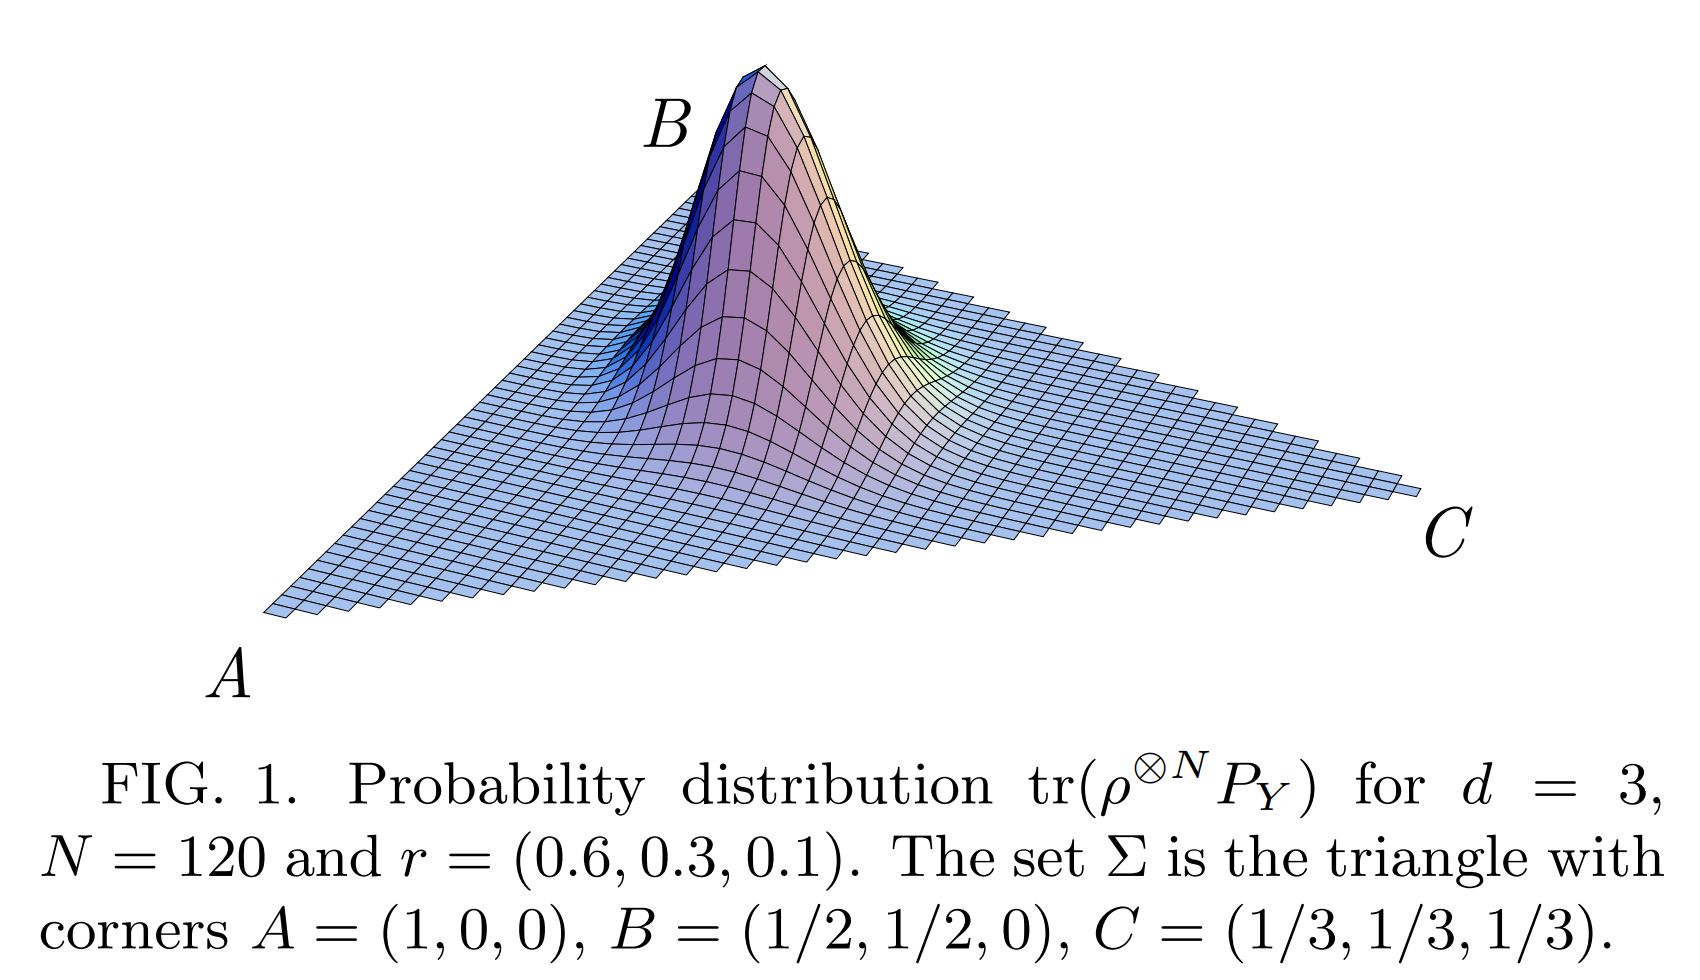
\includegraphics[width=\textwidth]{figures/keyl_werner.png}
        \end{column}
    \end{columns}
    \footcitetext{keyl2005estimating} 
\end{frame}

\begin{frame}
    \frametitle{Spectral Estimation Using Representation Theory}
    \begin{itemize}
        \item Elegant proof by \citeauthor{christandl2006spectra}~\footfullcite{christandl2006spectra}
        \item Spectra of $\rho^{\otimes k}$ is \textit{invariant} under both the action of $SU(d)$ and of $S_k$
        \item Utilize Weyl-Schur duality indexed by partitions of $\lambda \in \mathcal Y_k$
            \[ (\mathbb C^{d})^{\otimes k} = \bigoplus_{\lambda \in \mathcal Y_k} \mathcal U_{\lambda} \otimes \mathcal V_{\lambda} \]
        where $\mathcal U_{\lambda}$ and $\mathcal V_{\lambda}$ are irreps of $S_k$ and $SU(d)$ respectively
        \item Young diagrams $\mathcal Y_k$ describe partitions of $k$
            \begin{alignat*}{2}
                &\mathcal Y_1 = {\tiny\{ \yng(1) \}},
                &&\qquad\mathcal Y_2 = {\tiny\{ \yng(2),\yng(1,1) \}}, \\
                &\mathcal Y_3 = {\tiny\{ \yng(3),\yng(2,1),\yng(1,1,1) \}}
                &&\qquad\mathcal Y_4 = {\tiny\{ \yng(4),\yng(3,1),\yng(2,2),\yng(2,1,1),\yng(1,1,1,1) \}}, \ldots
            \end{alignat*}
        \item The eigenvectors of $\rho^{\otimes k}$ which are ``sufficiently symmetric'' are annihilated by the Young projection $P_{\lambda}$ onto the subspace $\mathcal U_\lambda \otimes \mathcal V_\lambda \subset (\mathbb C^d)^{\otimes k}$ 
    \end{itemize}
\end{frame}

\begin{frame}
    \frametitle{How to Survive a Young Projector}
    \begin{itemize}
        \item Eigen-decomposition of $\rho = {\sum}_{j=1}^{d} r_j \ket{v_j} \bra{v_j}$
        \item Eigenvectors of $\rho^{\otimes k}$ are then of the form
            \[ \ket{V_{J}} \coloneqq \ket{V_{(j_1, \ldots, j_k)}} \coloneqq \ket{v_{j_1}}\otimes\ket{v_{j_2}}\otimes \cdots \otimes\ket{v_{j_k}}\qquad J \in \{ 1, \ldots, d\}^{k} \]
        \item Example for $1 \leq i, j \leq d$ and $k=3$ with $\lambda = [1,1,1] \simeq \scalebox{0.4}{\yng(1,1,1)}$:
            \[ P_{\scalebox{0.4}{\yng(1,1,1)}} \ket{V_{(i, i, j)}} \propto \ket{V_{(i, i, j)}} - \ket{V_{(i, i, j)}} + \ket{V_{(i, j, i)}} - \ket{V_{(i, j, i)}}+\ket{V_{(j, i, i)}} - \ket{V_{(j, i, i)}} = 0\]
        \item Similar example for $1 \leq i, j \leq d$ and $k=4$ with $\lambda = [2,1,1] \simeq \scalebox{0.4}{\yng(2,1,1)}$:
            \[ P_{\scalebox{0.4}{\yng(2,1,1)}} \ket{V_{(i, i, j, j)}} \propto \ket{V_{(i, i, j, j)}} - \ket{V_{(i, i, j, j)}} + \cdots = 0\]
        \item Eigenvectors of $\rho^{\otimes k}$ which are ``too symmetric'' are annihilated!
    \end{itemize}
\end{frame}

\begin{frame}
    \frametitle{How to Survive a Young Projector, Cont'd}
    \begin{itemize}
        \item For $J \in \{1, \ldots, d\}^{k}$ define the \textit{multiplicity partition} $\mu(J) \in \mathcal Y_k$ in the obvious way:
            \[ \mu((1,1,2,4,4,4)) = [3, 2, 1] \simeq \scalebox{0.4}{\yng(3,2,1)} \]
    \end{itemize}
    \begin{theorem}
        Let $\ket{V_J}$ be a non-zero eigenvector of $\rho^{\otimes k}$ with \textit{multiplicity partition} $\mu(J) \in \mathcal Y_k$. Then
        \[ P_\lambda \ket{V_J} = 0 \iff \mu(J) \preceq \lambda \]
    \end{theorem}
    \begin{itemize}
        \item Where $\preceq$ is the \textit{majorization preorder} defined on partitions of $k$ as
            \[ \mu \preceq \lambda \iff \begin{cases} \sum_{i=1}^{m} \mu_{i} \leq \sum_{i=1}^{m} \lambda_{i} & \forall m \leq k-1, \\ \sum_{i=1}^{k} \mu_{i} = \sum_{i=1}^{k} \lambda_{i} \end{cases} \]
        where $\mu_1 \geq \mu_2 \geq \cdots \geq 0$ and $\lambda_1 \geq \lambda_2 \geq \cdots \geq 0$.
        \item As a corollary, eigenvalues of $P_\lambda \rho^{\otimes k} P_{\lambda}$ are upper bounded by $\prod_{i} r_i^{\lambda_i}$ (which is largest for $\lambda_i/k \approx r_i$)
    \end{itemize}
\end{frame}

\begin{frame}
    \frametitle{Hasse Diagrams for the Majorization Preorder of Partitions}
    \begin{columns}
        \begin{column}{0.25\textwidth}
            \begin{center}
                $k=1$ \\
                
\includegraphics[scale=0.4]{figures/majorization_k_1.pdf} \\
                \vspace{1em}
                $k=2$ \\
                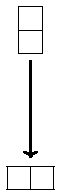
\includegraphics[scale=0.4]{figures/majorization_k_2.pdf} \\
                \vspace{1em}
                $k=3$ \\
                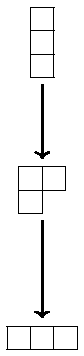
\includegraphics[scale=0.4]{figures/majorization_k_3.pdf}
            \end{center}
        \end{column}
        \begin{column}{0.25\textwidth}
            \begin{center}
                $k=4$ \\
                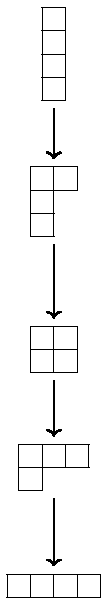
\includegraphics[scale=0.4]{figures/majorization_k_4.pdf}
            \end{center}
        \end{column}
        \begin{column}{0.25\textwidth}
            \begin{center}
                $k=5$ \\
                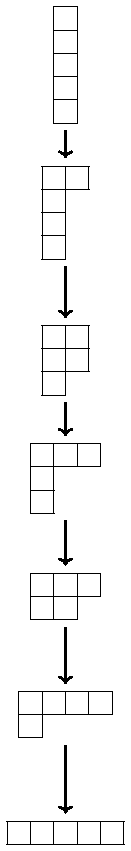
\includegraphics[scale=0.4]{figures/majorization_k_5.pdf}
            \end{center}
        \end{column}
        \begin{column}{0.25\textwidth}
            \begin{center}
                $k=6$ \\
                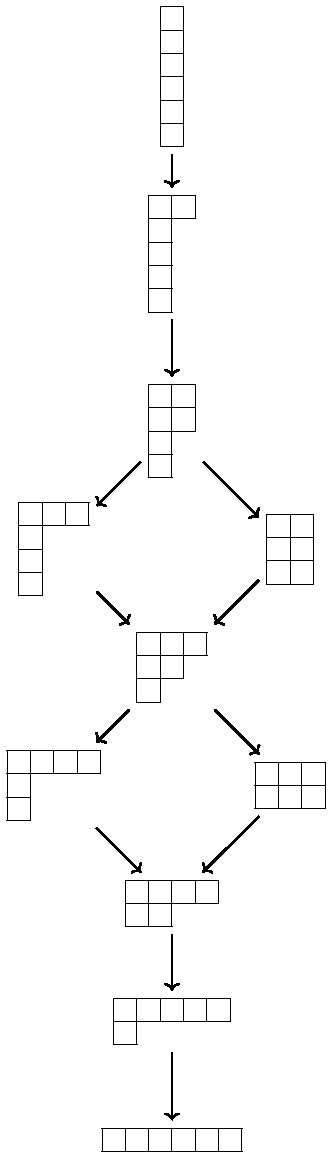
\includegraphics[scale=0.4]{figures/majorization_k_6.pdf}
            \end{center}
        \end{column}
    \end{columns}
\end{frame}

\begin{frame}
    \frametitle{Products of Density Operators and Where to Find Them}
    \begin{theorem}[\citeauthor{christandl2006spectra}~\citeyear{christandl2006spectra}]
        Let $\rho$ be a density operator with spectrum $r = \mathrm{spec}(\rho)$ and let $P_\lambda$ be the projection onto $\mathcal U_\lambda \otimes \mathcal V_\lambda$ for $\lambda \in \mathcal Y_k$. Then
        \[ \Tr ( P_\lambda \rho^{\otimes k} ) \leq (k + 1)^{d(d-1)/2} \exp ( - k D(\bar \lambda || r  )) \]
        where $\bar \lambda$ is defined as $\bar \lambda_i = \lambda_i / k$.
    \end{theorem}
    \begin{definition}[KL Divergence]
        The Kullback-Liebler divergence $D(p ||q)$ between two normalized probability distributions $p$ and $q$ is
        \[ D(p || q) = {\sum}_{i} p_i ( \log p_i - \log q_i ). \]
    \end{definition}
    \begin{itemize}
        \item Apply this result to the spectral QMP $\{ r_{AB}, r_{A}, r_{B} \}$
        \item Rough conclusion: for each $k$, there must be three partitions $\lambda, \mu, \nu$ of $k$ with
            \[ \bar \lambda \approx r_{AB}, \quad \bar \mu \approx r_{A}, \quad \bar \nu \approx r_{B} \]
            such that $(P_{\mu} \otimes P_{\nu}) P_{\lambda} \neq 0$
    \end{itemize}
\end{frame}

\begin{frame}
    \frametitle{Asymptotics of Kronecker Coefficients \& the Spectral Marginal Problem}
    \begin{definition}
        The \textit{Kronecker coefficients} dictate the irreps of $S_k$ which are sub-representations of products of irreps of $S_k$:
        \[ \mathcal U_{\mu} \otimes \mathcal U_{\nu}  = {\bigoplus}_{\lambda \in \mathcal Y_k} g_{\lambda \mu \nu} U_{\lambda} \]
    \end{definition}
    \begin{theorem}[Christandl-Mitchison, 2006]
        For every density operator $\rho_{AB}$, there is a sequence $(\lambda_j, \mu_j, \nu_j)$ of partitions with $j \in \mathbb N_+$ of $k_j = |\lambda_j| = |\mu_j| = |\nu_j|$ such that 
        \[ g_{\lambda_j \mu_j \nu_j} \neq 0 \quad \text{i.e.} \quad \mathcal U_{\lambda_j} \subset \mathcal U_{\mu_j} \otimes \mathcal U_{\nu_j} \]
        \begin{align*}
            \lim_{j\to \infty} \bar \lambda_j = \mathrm{spec}(\rho_{AB}), \qquad 
            \lim_{j\to \infty} \bar \mu_j = \mathrm{spec}(\rho_{A}), \qquad
            \lim_{j\to \infty} \bar \nu_j = \mathrm{spec}(\rho_{B}).
        \end{align*}
    \end{theorem}
    \begin{alertblock}{}
        \textit{``Calculation of the Kronecker coefficients is a tricky problem, arguably considered as `... the last major problem in ordinary representation theory of $S_k$' -- Yoav Dvir.''}
        \hspace*\fill{\small--- A. Klyachko}
    \end{alertblock}
\end{frame}

\section{Results about Overlapping QMP}
\begin{frame}
    \frametitle{Bipartite Entanglement \& Symmetric Extensions}
    \begin{itemize}
        \item The separability of a bipartite state $\rho_{AB} = {\sum}_{j} p_j \sigma_A^{(j)}\otimes \sigma_B^{(j)}$ can encoded as quantum marginals problem
            \[ \incstr{bipartite.pdf} = \incstr{sep_class_wire.pdf} .\]
        \item Assuming separability, there must exist a new state $\rho_{AB_1B_2\cdots B_k}$ called the \textit{$k$-symmetric extension} of $\rho_{AB}$ defined by
            \[ \incstr{kpartite.pdf} \coloneqq \incstr{sep_ext_k.pdf}. \]
        \item The $k$-symmetric extension has $\rho_{AB_i}$ marginals equal to $\rho_{AB}$ for all $i$:
            \[ \incstr{bipartite.pdf} \simeq \incstr{kpartite_marg.pdf}, \qquad \incstr{kpartite.pdf} \simeq \incstr{kpartite_sym.pdf}. \]
    \end{itemize}
\end{frame}

\begin{frame}
    \frametitle{A Complete Hierarchy of Separability Tests}
    \begin{theorem}[Doherty-Parrilo-Spedalieri, 2004]
        A bipartite mixed state $\rho$ on $\mathcal H_A \otimes \mathcal H_B$ is separable if and only if $\rho$ has a symmetric extension to $k$ copies for any and all $k$.
    \end{theorem}
    \footcitetext{doherty2004complete}
    \begin{theorem}[Chen-Ji-Kribs-Lütkenhaus-Zeng, 2014]
        A bipartite qubit mixed state $\rho$ on $\mathcal H_A \otimes \mathcal H_B$ admits of a $k=2$ symmetric extension if and only if
        \[ \Tr(\rho_{B}^2) \geq \Tr(\rho^2_{AB}) - 4 \sqrt{\det(\rho_{AB})}. \]
    \end{theorem}
    \begin{itemize}
        \item Serves as first analytic complete solution to an overlapping quantum marginals problem (as far as I know).
        \item Can be written entirely in terms of spectra:
        \[ {\sum}_{j}(\lambda_j^{B})^2 \geq {\sum}_{i}(\lambda_i^{AB})^2 - 4 \left({\prod}_{i} \lambda_i^{AB}\right)^{1/2}. \]
    \end{itemize}
    \footcitetext{chen2014symmetric}
\end{frame}

\begin{frame}
    \frametitle{Quantum Causality \& The Future of Marginal Problems}
    \begin{itemize}
        \item The ability to test causal hypotheses is intrinsically important to science
        \item For quantum theory, the quantum inflation technique due to \citeauthor{wolfe2019quantum}\footnotemark{} transforms quantum causal hypotheses into QMPs
        \item Quick example with \textit{triangle network}:
            \[ \incstr{triangle_state.pdf} = \incstr{triangle_production.pdf} \]
        \item The tripartite quantum state $\rho_{ABC}$ can be prepared using the triangle network only if there exists a $6$-partite quantum state $\Gamma_{A_1B_1C_1A_2B_2C_2}$ admitting certain marginals
    \end{itemize}
    \footcitetext{wolfe2019quantum}
\end{frame}

\begin{frame}
    \frametitle{A QMP for Triangle Network Compatibility}
    \begin{itemize}
        \item If $\rho_{ABC}$ is triangle network compatible,
    \end{itemize}
    \[ \incstr{triangle_state.pdf} = \incstr{triangle_production.pdf} \]
    \begin{itemize}
        \item then prepare $\rho_{ABC}$ twice,
    \end{itemize}
    \[ \incstr{triangle_state.pdf}\hspace{0.5em}\incstr{triangle_state.pdf} = \incstr{triangle_production_double.pdf} \]
    \begin{itemize}
        \item but instead rewire the sources,
    \end{itemize}
    \[ \incstr{triangle_sextuple.pdf} = \incstr{triangle_production_ring.pdf} \]
    \[ \incstr{triangle_sextuple.pdf} = \incstr{triangle_sextuple_swap.pdf} \]
\end{frame}

\begin{frame}
    \frametitle{A QMP for Triangle Network Compatibility, Cont'd}
    \begin{itemize}
        \item Some marginals of $\Gamma_{A_1B_1C_1A_2B_2C_2}$ are constrained by $\rho_{ABC}$,
    \end{itemize}
    \begin{align*}
        \incstr{triangle_sextuple_discard.pdf} 
        &= \incstr{triangle_production_ring_discard.pdf} \\
        &= \incstr{triangle_production_ring_discard_pulldown.pdf} \\
        &= \incstr{triangle_marg_state_Ac.pdf} \hspace{0.5em}\incstr{triangle_marg_state_Ac.pdf}
    \end{align*}
    \begin{align*}
        \Tr_{B_1B_2}(\Gamma_{A_1B_1C_1A_2B_2C_2}) &= \rho_{AC} \otimes \rho_{AC} \\
        \Tr_{A_1A_2}(\Gamma_{A_1B_1C_1A_2B_2C_2}) &= \rho_{BC} \otimes \rho_{BC} \\
        \Tr_{C_1C_2}(\Gamma_{A_1B_1C_1A_2B_2C_2}) &= \rho_{AB} \otimes \rho_{AB}
    \end{align*}
\end{frame}

\begin{frame}
    \frametitle{A QMP for Triangle Network Compatibility, Cont'd}
    \begin{align*}
        \incstr{triangle_sextuple_discard_3.pdf} 
        &= \incstr{triangle_production_ring_discard_3.pdf} \\
        &= \incstr{triangle_production_ring_discard_3_pulldown.pdf} \\
        &= \incstr{triangle_marg_state_A.pdf} \hspace{0.5em}\incstr{triangle_marg_state_C.pdf}\hspace{0.5em}\incstr{triangle_marg_state_B.pdf}
    \end{align*}
    \begin{align*}
        \Tr_{B_1A_2C_2}(\Gamma_{A_1B_1C_1A_2B_2C_2}) &= \rho_{A} \otimes \rho_{B} \otimes \rho_{C} \\
        \Tr_{A_1C_1B_2}(\Gamma_{A_1B_1C_1A_2B_2C_2}) &= \rho_{B} \otimes \rho_{A} \otimes \rho_{C}
    \end{align*}
\end{frame}

\section{References}
\begin{frame}[allowframebreaks]
    \frametitle{References}
    \printbibliography
\end{frame}


\end{document}
